\chapter{\IfLanguageName{dutch}{Stand van zaken}{State of the art}}%
\label{ch:stand-van-zaken}

% Tip: Begin elk hoofdstuk met een paragraaf inleiding die beschrijft hoe
% dit hoofdstuk past binnen het geheel van de bachelorproef. Geef in het
% bijzonder aan wat de link is met het vorige en volgende hoofdstuk.

% Pas na deze inleidende paragraaf komt de eerste sectiehoofding.
\section{\IfLanguageName{dutch}{Krachttraining}{Powerlifting}}%
\label{sec:krachttraining}

Krachttraining omvat intensieve oefeningen die het lichaam blootstellen aan hoge fysieke eisen en zware belastingen. 
Dit kan leiden tot blessures ten gevolge van overbelasting, verkeerde liftingtechnieken en onvoldoende rust.
De meeste blessures treden op tijdens de uitvoering van de squat, bench press en deadlift.  
Volgens \textcite{BengtssonEtAl2018} is het essentieel om de liftingtechniek te analyseren en te optimaliseren, evenals de trainingsbelasting en rusttijden, om het risico op blessures te verminderen.

\medskip

\subsection{\IfLanguageName{dutch}{Oefeningen}{Exercises}}%
\label{subsec:oefeningen}

De belangrijkste powerlifting-oefeningen zijn de squat, bench press en deadlift, die samen de basis van de sport vormen en de kwalificatie van de atleet bepalen. 
Elke oefening heeft specifieke kenmerken en technische vereisten. 

\medskip

Bij de \textbf{squat} staat de atleet met een halter op de schouders, zakt door de benen tot een bepaalde diepte en komt weer omhoog. 
Het doel is om het maximale gewicht te squatten, waarbij niet alleen de beenspieren, maar ook andere spieren, met name de rugspieren, betrokken zijn. 

\medskip

Bij de \textbf{bench press} ligt de atleet op een bank, laat een halter zakken tot de borst en drukt deze vervolgens weer omhoog.
Het doel is om het maximale gewicht te bankdrukken, waarbij technische aspecten zoals de positie van de voeten, schouders, gripbreedte en het neerlaten van de halter op de borst cruciaal zijn.

\medskip

De \textbf{deadlift} omvat het tillen van een halter van de grond tot een rechtopstaande positie met gestrekte rug en benen. 
Deze oefening wordt gezien als een indicator van absolute kracht in de rug en benen.

\subsection{\IfLanguageName{dutch}{Gevaren van een verkeerde liftingtechniek}{Dangers of an incorrect lifting technique}}%
\label{subsec:verkeerde-liftingtechniek}

De liftingtechniek is een cruciale factor bij powerliften en heeft een aanzienlijke invloed op het risico op blessures. 
Naast het managen van trainingsbelasting, is het optimaliseren van de liftingtechniek het belangrijkste preventieve middel tegen blessures \autocite{StrömbäckEtAl2018}.
Een suboptimale techniek is in verband gebracht met blessures, hoewel er onder onderzoekers, coaches en atleten discussie bestaat over wat een correcte techniek precies inhoudt. 
Hieronder worden de belangrijkste aspecten van de liftingtechniek bij de squat, bench press en deadlift besproken, evenals enkele algemene overwegingen.

\medskip

Bij de \textbf{squat} kunnen variaties in de techniek de krachten op de gewrichten beïnvloeden. 
Factoren zoals squatdiepte, standbreedte, bewegingssnelheid, barbellpositie en blikrichting spelen een rol bij het blessurerisico. 
Een grotere knieflexie verhoogt bijvoorbeeld de compressie- en schuifkrachten, terwijl valgus stress (knie flexie, heup adductie en interne rotatie van de femur) een punt van aandacht is. 
Een te brede stand kan de compressiekrachten op de knie verhogen, terwijl een smalle stand de anterieure schuifkrachten kan vergroten. 
Een hogere liftsnelheid of een stuiterende beweging onderaan de squat verhoogt de schuifkrachten op de knie, terwijl een snelle en ongecontroleerde afdaling de spanning op de kruisbanden en collaterale ligamenten kan vergroten. 
Daarnaast is een grotere voorwaartse leun geassocieerd met verhoogde lumbale schuifkrachten, en een hoge barbellpositie verplaatst de belasting van de heupen naar de knieën. 
Een neerwaartse blik kan de heupflexie en rompflexie vergroten.

\medskip

Bij de \textbf{bench press} wordt de oefening vaak gezien als een risicofactor voor schouderblessures. 
Factoren zoals gripbreedte, schouderpositie en het al dan niet trekken van een boog in de rug kunnen het blessurerisico beïnvloeden. 
Een brede grip kan de schouder in een nadelige positie plaatsen, wat belasting geeft aan het acromioclaviculaire gewricht, de glenohumerale ligamenten en de pectoralis major spier. 
Een wijdere grip verhoogt ook de schoudertorsie, wat de eisen aan de rotator cuff en bicepspees complex vergroot. 
Het verliezen van controle over de barbell kan leiden tot fracturen en schouderdislocaties.

\medskip

Bij de \textbf{deadlift} wordt een rechte torso met behoud van lumbale lordose verondersteld het blessurerisico te verminderen. 
Het dicht bij het lichaam houden van de barbell is belangrijk, omdat dit de heup- en spinale momentarmen verkleint en zo de prestaties verbetert en het blessurerisico vermindert. 
Het is ook essentieel om de knieën niet voortijdig of overmatig te strekken om een 'stiff-leg' deadlift te voorkomen. 
Bij de sumo-stijl kan de lifter een meer rechtopstaande torso behouden, wat het gemakkelijker maakt om de lumbale lordose te behouden. 
Deze stijl vermindert het L4/L5 moment en de schuifkrachten vergeleken met de conventionele stand.

\medskip

Naast de specifieke technieken per oefening zijn er algemene overwegingen. 
De combinatie van zware lasten en een onjuiste techniek verhoogt het blessurerisico aanzienlijk. 
Vermoeidheid kan de techniek negatief beïnvloeden, en het is belangrijk om te analyseren of een bewegingspatroon een adaptieve of maladaptieve reactie op pijn is. 
Het optimaliseren of veranderen van het bewegingspatroon kan pijn verminderen, en als dit het geval is, moeten de onderliggende bewegingssysteemstoornissen die het niet-optimale patroon veroorzaken, worden hersteld. 
Dit benadrukt het belang van technische precisie en aanpassing aan individuele behoeften om blessures te voorkomen en prestaties te optimaliseren \autocite{TymchikEtAl2021}.



\section{\IfLanguageName{dutch}{Artificiële Intelligentie}{Artificial Intelligence}}%
\label{sec:artificiële-intelligentie}

Artificiële Intelligentie (AI) is een dynamisch en snel evoluerend vakgebied dat zich richt op het ontwikkelen van systemen die taken kunnen uitvoeren die normaal gesproken menselijke intelligentie vereisen, zoals leren, probleemoplossing en besluitvorming \autocite{SharifaniEtAl2023}.

Het doel is om machines te ontwikkelen die autonoom kunnen functioneren in complexe en dynamische omgevingen \autocite{Kouassi2023}.

AI als vakgebied is al meer dan 65 jaar in ontwikkeling en heeft zich inmiddels diep genesteld in ons dagelijks leven. Het speelt immers een curicale rol in sectoren zoals gezondheidszorg, transport, onderwijs en industrie, en wordt gezien als een belangrijke drijfveer voor sociaaleconomische veranderingen en technologische vooruitgang \autocite{JiangEtAl2022}.

Binnen AI zijn Machine Learning (ML) en Deep Learning (DL) twee van de meest revolutionaire technologieën, die de afgelopen jaren aanzienlijke vooruitgang hebben geboekt \autocite{SharifaniEtAl2023}.

\section{\IfLanguageName{dutch}{Machine Learning}{Machine Learning}}%
\label{sec:machine-learning}

ML is momenteel de meest dominante vorm van AI. Het is een methode voor data-analyse die het mogelijk maakt om analytische modellen automatisch te bouwen en te verbeteren. Het stelt computers in staat om te leren van ervaring, zonder expliciet te worden geprogrammeerd \autocite{SharifaniEtAl2023}.

ML omvat de volgende technieken, die gecombineerd kunnen worden om nog krachtigere en veelzijdigere AI-systemen te ontwikkelen \autocite{Kouassi2023}. 

\begin{itemize}
  \item \textbf{Supervised Learning (SL)}: Hierbij wordt een model getraind met behulp van gelabelde gegevens, waarbij zowel de invoer als de gewensteuitvoer bekend zijn. Het model leert in feite door voorbeelden, vergelijkbaar met een leerling die oefent met vragen en de bijbehorende antwoorden. Het doel is om patronen te herkennen die vervolgens kunnen worden gebruikt om voorspellingen te maken voor nieuwe, onbekende gegevens. Voorbeelden van toepassingen zijn het herkennen van spam en het classificeren van afbeeldingen.
  \item \textbf{Unsupervised Learning (UL)}: Deze techniek werkt met ongelabelde data, waarbij het model zelf patronen of structuren moet ontdekken. Dit gebeurt vaak door clustering, waarbij vergelijkbare data automatisch worden gegroepeerd. Een voorbeeld is het segmenteren van klanten op basis van koopgedrag. UL is vooral nuttig wanneer er geen duidelijke labels beschikbaar zijn. 
  \item \textbf{Reinforcement Learning (RL)}: RL draait om een model dat leert door interactie met een omgeving. Het model probeert een strategie (beleid) te ontwikkelen die maximale beloningen oplevert. Dit wordt vaak gebruikt in scenario's zoals robotica, gaming en autonome voertuigen, waarbij het model leert door trial-and-error. 
\end{itemize}

\begin{figure}
  \centering
  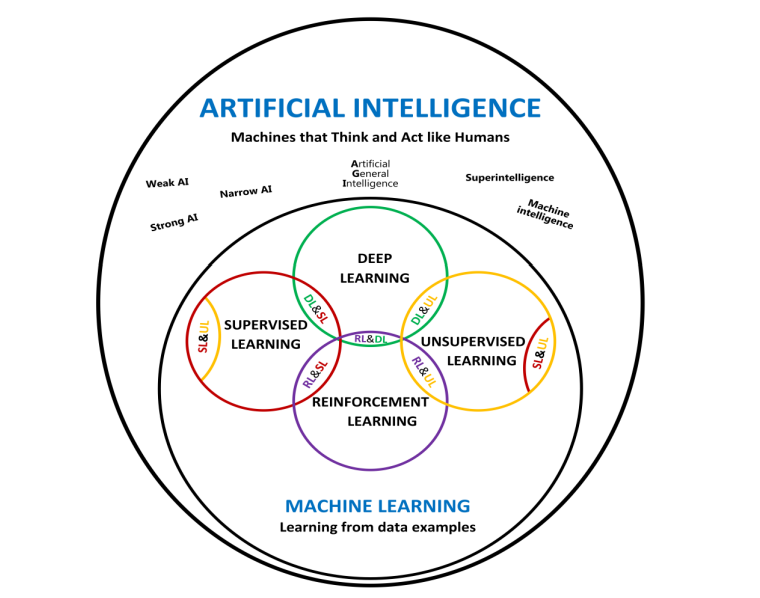
\includegraphics[width=0.8\textwidth]{ai.png}
  \caption[Figuur 1]{\label{fig:ai}Het AI landschap met zijn verschillende technieken \autocite{Kouassi2023}}
\end{figure}

\section{\IfLanguageName{dutch}{Deep Learning}{Deep Learning}}%
\label{sec:deep-learning}

Dit is een geavanceerde vorm van ML die gebruikmaakt van gelaagde neurale netwerken, geïnspireerd op de structuur van het menselijk brein.
Het model verwerkt data iteratief, waarbij het parameters aanpast op basis van feedback.  
Het is vooral geschikt voor taken met grote hoeveelheden ongestructureerde data, zoals beeld- en spraakherkenning. 
In tegenstelling tot traditionele ML modellen kan DL automatisch hoogwaardige kenmerken uit data halen, waardoor het beter presteert bij ingewikkelde taken \autocite{SharifaniEtAl2023}.

Er zijn verschillende DL-architecturen, zoals Convolutionele Neurale Netwerken (CNN's) voor beeldverwerking en Recurrente Neurale Netwerken (RNN's) voor tijdreeksdata. 
DL kan zowel end-to-end systemen vormen als kenmerken extraheren voor andere ML-modellen \autocite{JanieschEtAl2021}. 

Kortom, Deep Learning is een krachtige en veelzijdige technologie die een centrale rol speelt in de moderne AI-revolutie. 
Het is bijzonder effectief in het verwerken van grote en complexe datasets en heeft toepassingen in tal van domeinen. 
Echter, de ontwikkeling van DL-modellen brengt ook uitdagingen met zich mee, zoals het optimaliseren van modellen en het integreren van logisch redeneren. 
DL blijft een belangrijk onderzoeksgebied met een groot potentieel voor toekomstige innovaties \autocite{JiangEtAl2022}.

\section{\IfLanguageName{dutch}{Computer Vision}{Computer Vision}}%
\label{sec:computer-vision}

Computer Vision (CV) is een snelgroeiend vakgebied binnen de beeldverwerking, waarbij CNN's, een belangrijk onderdeel van DL, een centrale rol spelen.  

In de beginfase van CV werden DL-methoden beperkt door technische uitdagingen, zoals beperkt geheugen en rekenkracht. 
Hierdoor lag de focus aanvankelijk op traditionele ML-technieken. 
Met de verbetering van hardware (CPU/GPU) en de ontwikkeling van krachtige DL-modellen werd DL echter de dominante benadering in CV \autocite{ChaiEtAl2021}.

CNN's hebben een revolutie teweeggebracht in taken zoals beeldclassificatie, objectdetectie en beeldreconstructie. 
Ze leren automatisch kenmerken uit ruwe data, waardoor ze complexe patronen kunnen herkennen en hogere niveau-representaties kunnen vormen. 
Dit maakt ze ideaal voor praktische toepassingen. 

CV wordt breed ingezet in domeinen zoals autonoom rijden (object- en verkeersherkenning), virtual reality (immersieve ervaringen), en intelligente videobewaking (detectie van verdachte activiteiten). 
Ook wordt het gebruikt voor Human Activity Recognition (HAR), zoals het monitoren van ouderen of revalidatie, en voor taken zoals spraakherkenning en sentimentanalyse. 

Een belangrijke uitdaging is dat CNN's veel rekenkracht en grote hoeveelheden gelabelde data vereisen, wat kostbaar en tijdrovend kan zijn. 
Toch blijft het veld zich snel ontwikkelen, met toekomstige richtingen zoals ensemble learning (combinatie van meerdere CNN's), aandachtsmechanismen (gericht op belangrijke informatie in beelden) \autocite{ZhaoEtAl2024}. 

\section{\IfLanguageName{dutch}{Pose Estimation}{Pose Estimation}}%
\label{sec:pose-estimation}
 
Pose Estimation is een CV-techniek die menselijke poses schat door lichaamsdelen en gewrichtsposities te detecteren in afbeeldingen of video's. 
Het wordt gebruikt in toepassingen zoals games, animatie, medische analyse, AI-gestuurde persoonlijke trainers, human-computer interactie, bewegingsanalyse, augmented reality, virtual reality, posetracking, actieherkenning en surveillance systemen \autocite{SiddharthEtAl2021}.

Er zijn twee hoofdbenaderingen: single-person (één persoon per frame) en multi-person (meerdere personen, inclusief occlusies). 
Methoden variëren van top-down (eerst personen detecteren, dan lichaamsdelen) tot bottom-up (eerst lichaamsdelen detecteren, dan toewijzen aan personen). 
Pose estimation kan in 2D (gewrichtslocaties in 2D) of 3D (ruimtelijke opstelling van gewrichten) worden uitgevoerd. 
3D HPE is toepasbaar in virtual reality en sportanalyse en kan single-view (één camerabeeld) of multi-view (meerdere camerabeelden om occlusies te overwinnen) zijn \autocite{ZhengEtAl2023}.

Convolutional Neural Networks (CNN's) spelen een centrale rol, waarbij ze worden getraind om lichaamsdelen te classificeren en ruimtelijke modellen te combineren voor nauwkeurige resultaten. 
Andere geavanceerde technieken zijn Transformers (voor langeafstandsafhankelijkheden), Graph Convolutional Networks (voor correlaties tussen gewrichten) en Adversarial Learning (om robuustheid en nauwkeurigheid te verbeteren). 
Moderne methoden zoals DeepPose (gebruikt Deep Neural Networks), Adversarial PoseNet (combineert generatoren en discriminatoren voor nauwkeurige heatmaps) en OpenPose (real-time multi-person schatting met Part Affinity Fields) hebben het veld aanzienlijk vooruit geholpen \autocite{ZhaoEtAl2024}.

Een van de grootste uitdagingen bij HPE is het verlies van low-level kenmerken, beperkte receptive fields, en problemen veroorzaakt door occlusies of verstrengelde lichaamsdelen. 
Om deze problemen aan te pakken, worden attention mechanisms zoals Context Coordinate Attention Module (CCAM), channel attention en spatial attention gebruikt om de aandacht te richten op belangrijke lichaamsdelen voor nauwkeurigere resultaten. 
Populaire modellen zoals YOLOv8x-pose combineren snelheid en precisie, waardoor ze geschikt zijn voor real-time toepassingen.

Voor training en evaluatie worden datasets zoals MS COCO 2017 (meer dan 20.000 afbeeldingen met 17 geannoteerde gewrichten) en CrowdPose (gericht op real-world crowd-scènes) gebruikt. 
Evaluatiemetrics omvatten Average Precision (AP), gebaseerd op Object Keypoint Similarity (OKS), Average Recall (AR) voor het meten van keypoint-herkenning, en Latency (ms) om de inference-tijd van het model te beoordelen \autocite{DongEtAl2024}.

Een voorbeeld van een geavanceerd model is CCAM-Person, gebaseerd op het YOLOv8-framework, dat YOLOv8 combineert voor doelherkenning met een binary classification-achtige benadering om keypoints te detecteren. Het model introduceert de Multi-scale Receptive Field (MRF) Module en het Multi-path Feature Pyramid Network (MFPN) om de interactie tussen verschillende feature-niveaus te optimaliseren, evenals het Context Coordinate Attention Module (CCAM) om de precisie te verhogen, vooral in gevallen van omgevingsgeluid of occlusies. 
Experimentele resultaten tonen aan dat CCAM-Person concurrerende prestaties behaalt, met een verbetering van 2.8\% in average precision en 4.2\% in recall rate op de MS COCO 2017-dataset, en een stijging van 3.5\% in AP op de CrowdPose-dataset. 
Ondanks een lichte afname in inference-snelheid door de aandachtmodules en multi-path fusie, blijft het model voldoen aan real-time eisen \autocite{DongEtAl2024}.

Kortom, Human Pose Estimation (HPE) is een veelzijdige techniek met brede toepassingen, ondersteund door geavanceerde modellen en aandacht voor uitdagingen zoals occlusies en schaalvariaties. 
Door de inzet van deep learning-technieken en innovatieve benaderingen blijft het veld zich snel ontwikkelen, met als doel real-time, nauwkeurige en robuuste pose-schatting mogelijk te maken \autocite{DongEtAl2024}.

Technologieën zoals OpenPose, PoseNet en MoveNet bieden groot potentieel voor toepassingen op mobiele apparaten. 
Deze methoden schatten poses door middel van deep learning op basis van camerainput, waardoor er geen extra sensoren nodig zijn en ze breed inzetbaar zijn op de meeste apparaten. 
Ondanks dat OpenPose ongeveer 12 keer langzamer is dan MoveNet, heeft het als voordeel dat het de poses van meerdere personen tegelijk kan schatten. PoseNet blinkt uit in nauwkeurigheid, terwijl MoveNet Lightning het snelste model is.
Deze technologieën openen de deur naar innovatieve toepassingen en verbeterde gebruikerservaringen op mobiele apparaten \autocite{BeomjunEtAl2022}.

OpenPose was het eerste model dat realtime poseschatting voor meerdere personen mogelijk maakte. 
OpenPose maakt gebruik van een bottom-up methode, waarmee het de beperkingen van de traditionele top-down aanpak overwint. 
Dit model schat poses via deep learning op basis van camerainput, waardoor er geen extra sensoren nodig zijn en het breed toepasbaar is op de meeste apparaten. 
Een belangrijk kenmerk van OpenPose is dat het de poses van meerdere personen tegelijk kan schatten. 
Het model ondersteunt 137 keypoints: 25 voor het lichaam (inclusief de voeten), 21 voor elke hand en 70 voor het gezicht.
OpenPose maakt gebruik van Part Affinity Fields (PAFs), een set van flow-velden die de relaties tussen lichaamsdelen van meerdere personen weergeven \autocite{KanaseEtAl2021}.  
Hoewel het model 12 keer langzamer is dan MoveNet, blinkt het uit in het nauwkeurig identificeren van meerdere personen en het schatten van hun poses binnen een afbeelding. 
Het herkent ook het verschil tussen objecten in één fase en vertoont een hoge prestatienauwkeurigheid.
OpenPose is een krachtig hulpmiddel voor realtime poseschatting, vooral in scenario's waarbij meerdere personen moeten worden geanalyseerd \autocite{BeomjunEtAl2022}.

PoseNet is een open source machine learning-model ontwikkeld door Google Creative Lab, ontworpen om menselijke poses in realtime te schatten. 
Het model maakt gebruik van de COCO person key-point detection dataset, die de belangrijkste punten van het hele lichaam volgt. 
Voor single-person poseschatting gebruikt PoseNet vier invoerelementen: een inputafbeelding, een image scale factor, een horizontale flip en een output stride. 
Het single-person detection algoritme is sneller en eenvoudiger dan het multi-person detection algoritme. 
PoseNet is ook beschikbaar voor mobiele apparaten via TensorFlow Lite, waardoor het compatibel is met Android en iOS. 
PoseNet maakt gebruik van de top-down methode, waarbij eerst een persoon wordt gedetecteerd en vervolgens de pose binnen de bounding box wordt geschat. 
Het model biedt in totaal 17 key-points: 5 in het gezicht en 12 in het lichaam. 
PoseNet behaalde de hoogste nauwkeurigheid en had de kleinste standaarddeviatie, wat wijst op een consistente prestatie tussen runs \autocite{BeomjunEtAl2022}.

MoveNet is een op Google gebaseerd inferentiemodel, ontwikkeld door IncludeHealth, een digitaal gezondheidsbedrijf.
Het model is beschikbaar in twee versies: een webversie die gebruikmaakt van TensorFlow.js en een mobiele versie die draait op TensorFlow Lite. 
MoveNet kent twee varianten: Lightning, gericht op prestaties, en Thunder, gericht op nauwkeurigheid. 
Lightning ontvangt een video of afbeelding van een vaste grootte (192\times192) met drie kanalen en gebruikt een dieptemultiplier van 1.0. 
Thunder daarentegen ontvangt een input van 256\times256 met drie kanalen en gebruikt een dieptemultiplier van 1.75, wat betekent dat het 1.75 keer meer lagen voor deep learning heeft en daardoor meer berekeningen uitvoert.
MoveNet is een bottom-up model dat gebaseerd is op CenterNet en alle vier processen gelijktijdig berekent. 
Het model biedt in totaal 17 key-points: 5 in het gezicht en 12 in het lichaam. 
MoveNet Lightning is het snelste model, terwijl Thunder zich onderscheidt door een hogere nauwkeurigheid \autocite{BeomjunEtAl2022}. 


\subsection{\IfLanguageName{dutch}{Uitdagingen van Pose Estimation op Mobiele Apparaten}{Challenges for Pose Estimation on Mobile Devices}}%
\label{subsec:uitdagingen-van-pose-estimation-op-mobiele-apparaten}
\begin{itemize}
    \item \textbf{Beperkte Rekenkracht}: 
    Mobiele apparaten hebben minder hardwarecapaciteit dan servers of computers, waardoor het gebruik van complexe en grote neurale netwerken moeilijk is. Pose estimation-algoritmen vereisen vaak veel rekenkracht, wat kan leiden tot trage prestaties en een hoog energieverbruik \autocite{LiuEtAl2022}.

    \item \textbf{Modelgrootte}: 
    Voor mobiele toepassingen moeten modellen compact zijn om efficiënt te kunnen draaien. Grote modellen zijn vaak niet geschikt vanwege beperkte opslag en geheugen op mobiele apparaten \autocite{HouEtAl2020}.

    \item \textbf{Real-time Prestaties}: 
    Pose estimation moet in real-time werken, vooral voor toepassingen zoals fitness-tracking of augmented reality. Vertragingen kunnen de gebruikerservaring negatief beïnvloeden \autocite{HouEtAl2020}.

    \item \textbf{Wisselende Omstandigheden}: 
    Mobiele apparaten worden in diverse omgevingen gebruikt, wat pose estimation uitdagend maakt. Factoren zoals camerarotaties, wisselende belichting, en occlusies (bijvoorbeeld wanneer lichaamsdelen elkaar overlappen) kunnen de nauwkeurigheid verminderen \autocite{SulongEtAl2023}.

    \item \textbf{Beperkte Trainingsdata}: 
    Het verzamelen van voldoende en gevarieerde trainingsdata is een uitdaging, wat de nauwkeurigheid van modellen kan beperken. Dit geldt vooral voor scenario’s met ongebruikelijke poses of achtergronden \autocite{PauloEtAl2024}.

    \item \textbf{Nauwkeurigheidsproblemen}: 
    Beeldvervorming, achtergrondruis of complexe objecten kunnen de nauwkeurigheid van pose estimation beïnvloeden. Dit is vooral problematisch bij objecten met ongebruikelijke vormen of structuren \autocite{SulongEtAl2023}.
\end{itemize}

Om de uitdagingen van pose estimation op mobiele apparaten het hoofd te bieden, zijn enkele praktische stappen nodig. Ten eerste is het belangrijk om een lichtgewicht model te kiezen dat minder rekenkracht vereist, maar toch goede prestaties levert. Dit maakt het mogelijk om real-time resultaten te behalen op mobiele hardware. Daarnaast moet het model getraind worden op diverse omstandigheden, zoals wisselende belichting, camerahoeken en occlusies, om de nauwkeurigheid in verschillende omgevingen te waarborgen.
\medskip
Ook is het nuttig om best practices voor training toe te passen, zoals het gebruik van synthetische data of transfer learning, vooral als er beperkte trainingsdata beschikbaar is. Dit helpt om het model robuuster en nauwkeuriger te maken. Ten slotte kan het gebruik van beschikbare tools en frameworks het proces vereenvoudigen, waardoor het trainen en implementeren van het model efficiënter verloopt.
